\section{Simulationen}
\hypertarget{Sec:Sim}{}

In diesem Kapitel werden wir uns mit der Simulation von Zufallsvariablen beschäftigen. Hierzu benötigen wir zunächst die folgende

\begin{Definition}{(Inverse Verteilungsfunktion) \cite{Nelson}}
Sei $(\Omega, \mathscr{A}, \mathbb{P})$ ein Wahrscheinlichkeitsraum und $X$ eine reelle Zufallsvariable mit Verteilungsfunktion $F_X$. Zu $p \in [0, 1]$ ist das \textit{$p$-Quantil} definiert durch
\[F_X^{-1}(p) := \inf\{ x \in \mathbb{R} \mid F_X(x) \geq p \}~.\]
Damit erhält man die \textit{inverse Verteilungsfunktion}
\[F_X^{-1}: [0, 1] \rightarrow \mathbb{R}: p \mapsto F_X^{-1}(p)~.\]
\end{Definition}

Mit dieser Definition können wir nun den Satz formulieren und beweisen, der die Grundlage unserer Simulationsmethode bilden wird.

\begin{Satz}{(Inversionsmethode) \cite{Nelson}}
Sei $(\Omega, \mathscr{A}, \mathbb{P})$ ein Wahrscheinlichkeitsraum und $X$ eine reelle Zufallsvariable mit Verteilungsfunktion $F_X$. Sei weiter $U$ auf $[0, 1]$ stetig gleichverteilt. Dann ist $F_X^{-1}(U)$ wieder eine reelle Zufallsvariable mit der gleichen Verteilung wie $X$.
\end{Satz}

\begin{Beweis}{\cite{Nelson}}
Nach Definition der inversen Verteilungsfunktion gilt insbesondere
\begin{align*}
F_X^{-1}(U) &\leq x
\intertext{genau dann, wenn}
U &\leq F_X(x)~.
\end{align*}
Betrachte zu $x \in \mathbb{R}$
\begin{align*}
\mathbb{P}(F_X^{-1}(U) \leq x) &= \mathbb{P}(U \leq F_X(x))~.
\intertext{Da $U$ auf $[0, 1]$ gleichverteilt ist, gilt nach dem \hyperlink{Bsp:VertFun}{\blue{Beispiel zur Berechnung von Verteilungsfunktionen}}}
&= F_X(x)~,
\end{align*}
denn $F_X(x) \in [0, 1]$ nach den \hyperlink{Satz:EigVertFun}{\blue{Eigenschaften der Verteilungsfunktion}}.
\end{Beweis}

\medskip

Diese Methode wollen wir gleich programmieren.

\begin{Code}{(\lstinline|simulate|)}
Aufgrund der unterschiedlichen Arten von Verteilungsfunktionen müssen wir diese Methode wieder für jeden Typen getrennt implementieren.
\begin{enumerate}[label=(\roman*)]
\item Für finite Zufallsvariablen gilt
\begin{lstlisting}
def simulate(self, number):
    simulate = []
    uni = np.random.uniform(0, 1, number)
    distribution_function = self.distribution_function()
    for num in uni:
        for key in distribution_function.keys():
            if num <= float(distribution_function[key]):
                simulate.append(float(key))
                break
    return simulate
\end{lstlisting}
Der erste Teil läuft für alle Typen gleich ab. Wir erzeugen mit NumPy ein Array von auf $[0, 1]$ gleichverteilten Zufallszahlen. Die Anzahl muss als Argument übergeben werden. Wir lassen uns anschließend die Verteilungsfunktion berechnen. Nun iterieren wir über alle gleichverteilten Werte und anschließend über alle kumulierten Wahrscheinlichkeiten, die unsere Verteilungsfunktion annimmt. Sobald wir das erste Mal mit dem gleichverteilten Wert kleiner sind, als die kumulierten Wahrscheinlichkeit, fügen wir den zugehörigen $x$-Wert der Verteilungsfunktion dem Simulationsergebnis hinzu und brechen die innere Schleife ab. Diese Methode funktioniert, da die $x$-Werte der Verteilungsfunktion im Dictionary sortiert sind und  wir so genau das Infimum finden.

\item Für diskrete Zufallsvariablen gilt
\begin{lstlisting}
def simulate(self, number, n_max=100):
    simulate = []
    n_list = [n for n in range(n_max) if n >= self.supp[0] and n <= self.supp[1]]
    uni = np.random.uniform(0, 1, number)
    for num in uni:
        cumulative_probability = sym.Integer(0)
        for n in n_list:
            cumulative_probability += self.density.subs(self.variable, n)
            if num <= cumulative_probability:
                simulate.append(n)
                break
    return simulate
\end{lstlisting}
Die Simulation für diskrete Zufallsvariablen läuft ganz ähnlich ab. Als zusätzliches Argument haben wir \lstinline|n_max|. Diese Zahl bestimmt, bis zu welchem Wert die kumulierte Wahrscheinlichkeit berechnet wird. Wir bilden zuerst eine Liste der ersten \lstinline|n_max| Zahlen, die in unserem Träger liegen. Anschließend iterieren wir wieder über jede der gleichverteilten Zahlen. Als nächstes durchlaufen wir die Liste der ersten \lstinline|n_max| Zahlen und bilden jeweils die kumulierte Wahrscheinlichkeit. Falls die kumulierte Wahrscheinlichkeit das erste Mal größer ist, als der gleichverteilte Wert, fügen wir das \lstinline|n| der Simulationsliste hinzu und brechen die innere Schleife ab. Da wir uns von unten an den gleichverteilten Wert herantasten, finden wir auf jeden Fall das Infimum. Sollte der gleichverteilte Wert sehr nahe an eins liegen, sorgt das \lstinline|n_max| dafür, dass die Schleife auf jeden Fall terminiert.

\item Für stetige Zufallsvariablen gilt
\begin{lstlisting}
def simulate(self, number):
    simulate = []
    uni = np.random.uniform(0, 1, number)
    t = sym.Symbol('t', real=True)
    distribution_function = self.distribution_function()
    mean = self.mean()
    for num in uni:
        eq = sym.Eq(distribution_function, num)
        sim = sym.nsolve(eq, t, mean)
        simulate.append(float(sim))
    return simulate
\end{lstlisting}
Diese Simulation läuft etwas anders ab. Wir lassen uns neben der Verteilungsfunktion noch den Erwartungswert berechnen. Somit muss der Erwartungswert endlich sein. Trotz dieser deutlichen Einschränkung ist diese Herangehensweise sehr sinnvoll, da alle Werte der Zufallsvariable um den Erwartungswert verteilt sind. Würden wir einen bestimmten Wert, wie zum Beispiel Null wählen, so wäre eine Normalverteilung mit $\mu = 10^6$ sehr schwierig zu simulieren, da der Abstand zwischen Startwert und gesuchtem Wert zum einen sehr groß ist und zum anderen die Steigung sehr klein wäre.

\newpage

Im nächsten Schritt der Simulation lösen wir für jeden Wert $u$ der Gleichverteilung die Gleichung
\[F(x) = u\]
nach $x$ auf. Symbolisch lässt sich diese Gleichung meistens leider nicht lösen. Als Startwert für die numerische Lösung verwenden wir den Erwartungswert. Dieser Algorithmus kann im stetigen Falle theoretisch für Verteilungsfunktionen, die nicht streng monoton wachsend sind, schiefgehen. Dies liegt daran, dass die numerische Approximation möglicherweise nicht den richtigen Wert \glqq findet\grqq{}. Hierzu werden wir gleich ein Beispiel betrachten.
\end{enumerate}

An dieser Stelle sei erwähnt, dass die oben implementierte Simulationsmethode keineswegs effizient implementiert ist. Wie an den meisten Stellen ist es hier leider nicht möglich große Laufzeitvorteile durch Vektorisierung zu erhalten, da es für viele Verteilungen nicht die Möglichkeit gibt die SymPy-Funktionen in beispielsweise NumPy-Funktionen zu übersetzen, um dort effizienter zu arbeiten.
\end{Code}

Nun betrachten wir eine Verteilungsfunktion, die vermutlich Probleme machen würde.

\begin{Beispiel}{(Nicht-simulierbare Zufallsvariable)}
Sei $X$ eine reelle Zufallsvariable mit der folgenden Verteilungsfunktion

\begin{figure}[H]
\centering
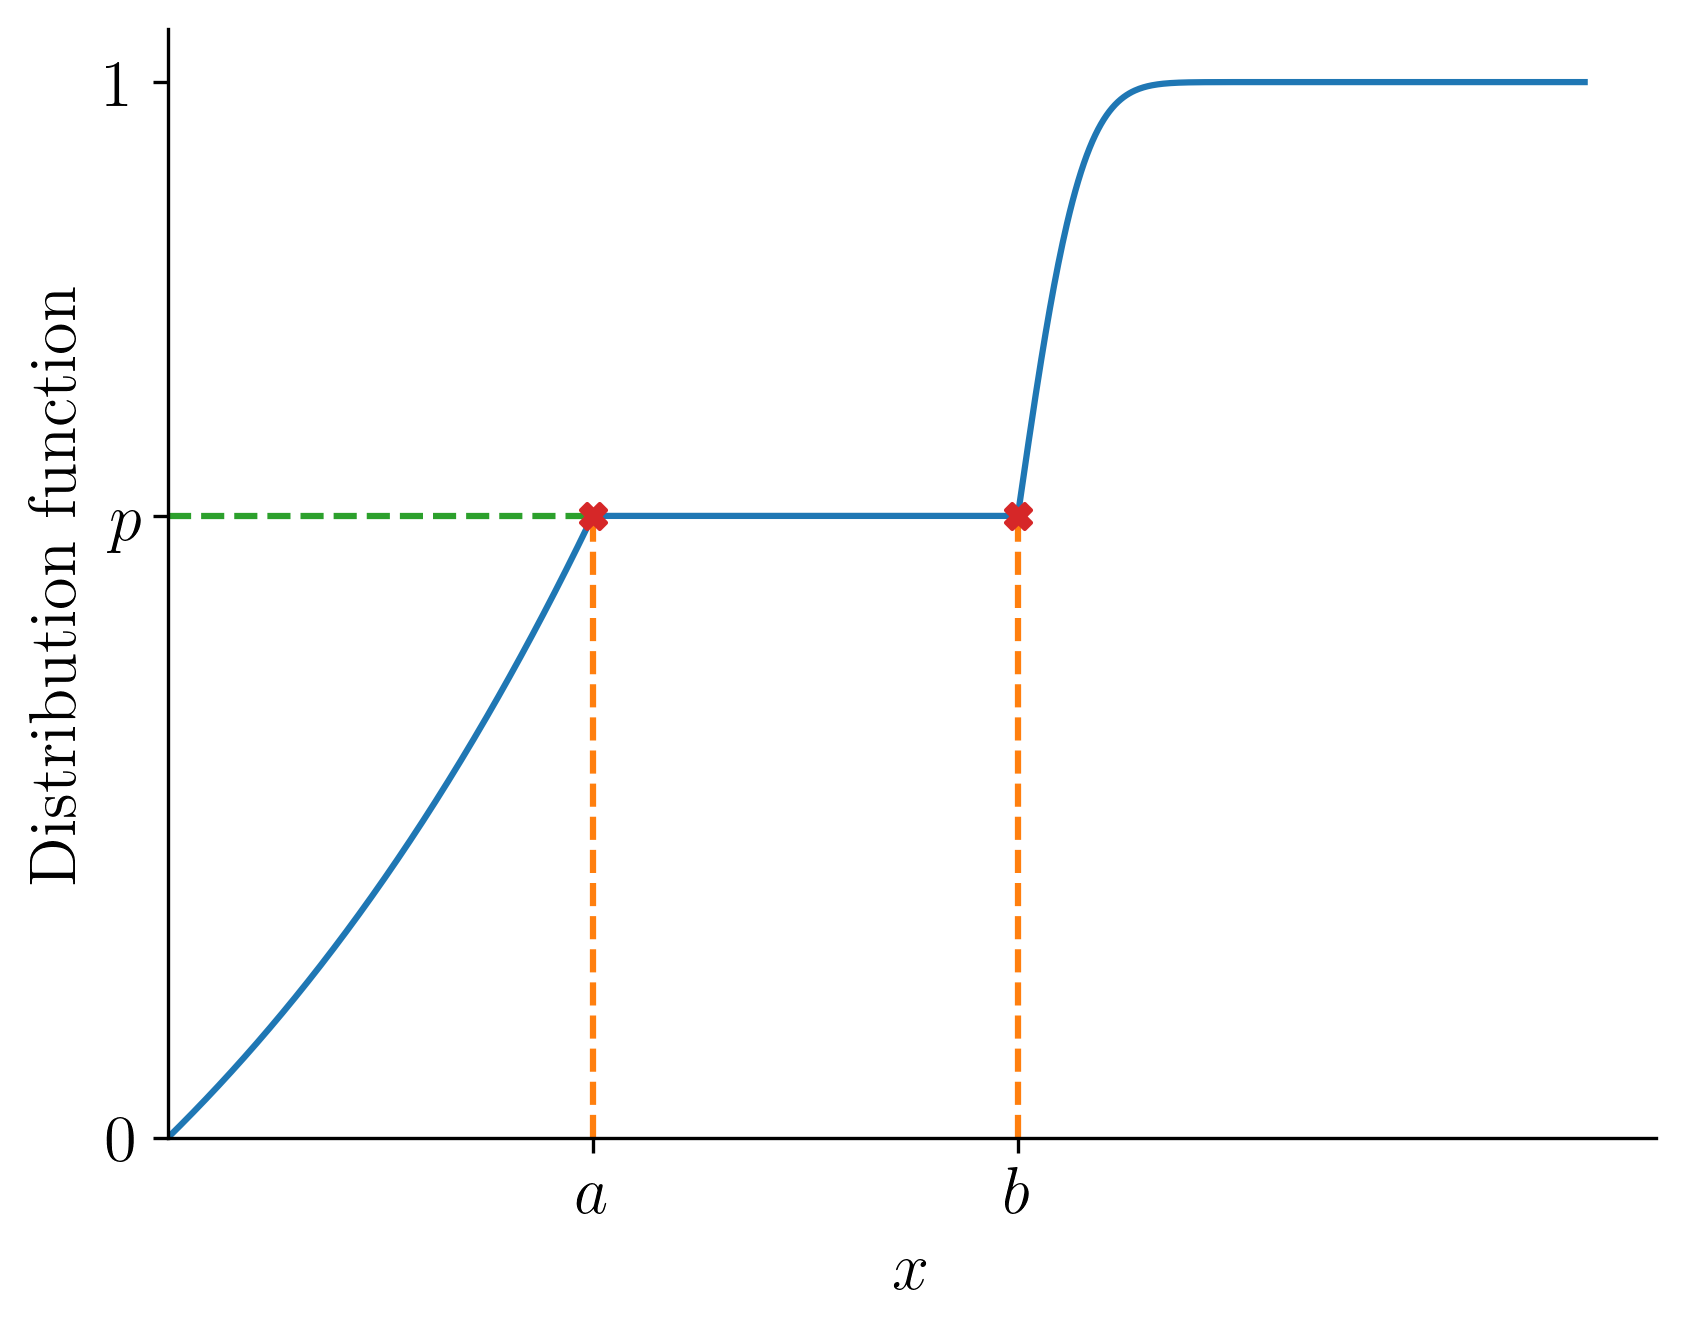
\includegraphics[width=0.5\linewidth]{./Section/Simulation/Nicht Simulierbar.png}
\caption{Verteilungsfunktion einer vermutlich schlecht simulierbaren Verteilung}
\end{figure}

Die Verteilungsfunktion ist auf $[a, b]$ nur monoton. Ist $U = p$, so ist
\begin{align*}
F^{-1}(p) &= \inf\{ x \in \mathbb{R} \mid F(x) \geq p\}\\
&= \inf\{ x \in [a, \infty)\}\\
&= a~.
\end{align*}
Die numerische Methode hingegen versucht ein $x \in \mathbb{R}$ zu finden mit $F(x) = p$ . Ist $\mathbb{E}(X) > b$, so findet die numerische Methode vermutlich zuerst den Wert $b$, womit wir dann ein falsches Ergebnis erhalten. In den allermeisten Fällen sollte dies jedoch gut gehen.
\end{Beispiel}

\newpage

Nun können wir einige Beispiele untersuchen, für die die Methode wunderbar funktioniert.

\begin{Beispiel}{(Klassische Zufallsvariablen)}
Um die Richtigkeit unserer Ergebnisse zu \glqq überprüfen\grqq{}, können wir unseren Code mit den entsprechenden Funktionen von NumPy vergleichen. Wir verwenden eine Bernoulli-Verteilung als finites, eine Poisson-Verteilung als diskretes, sowie eine Normal- und Exponentialverteilung als stetige Beispiele.\\
\begin{minipage}{0.5\linewidth}
\begin{figure}[H]
\begin{center}
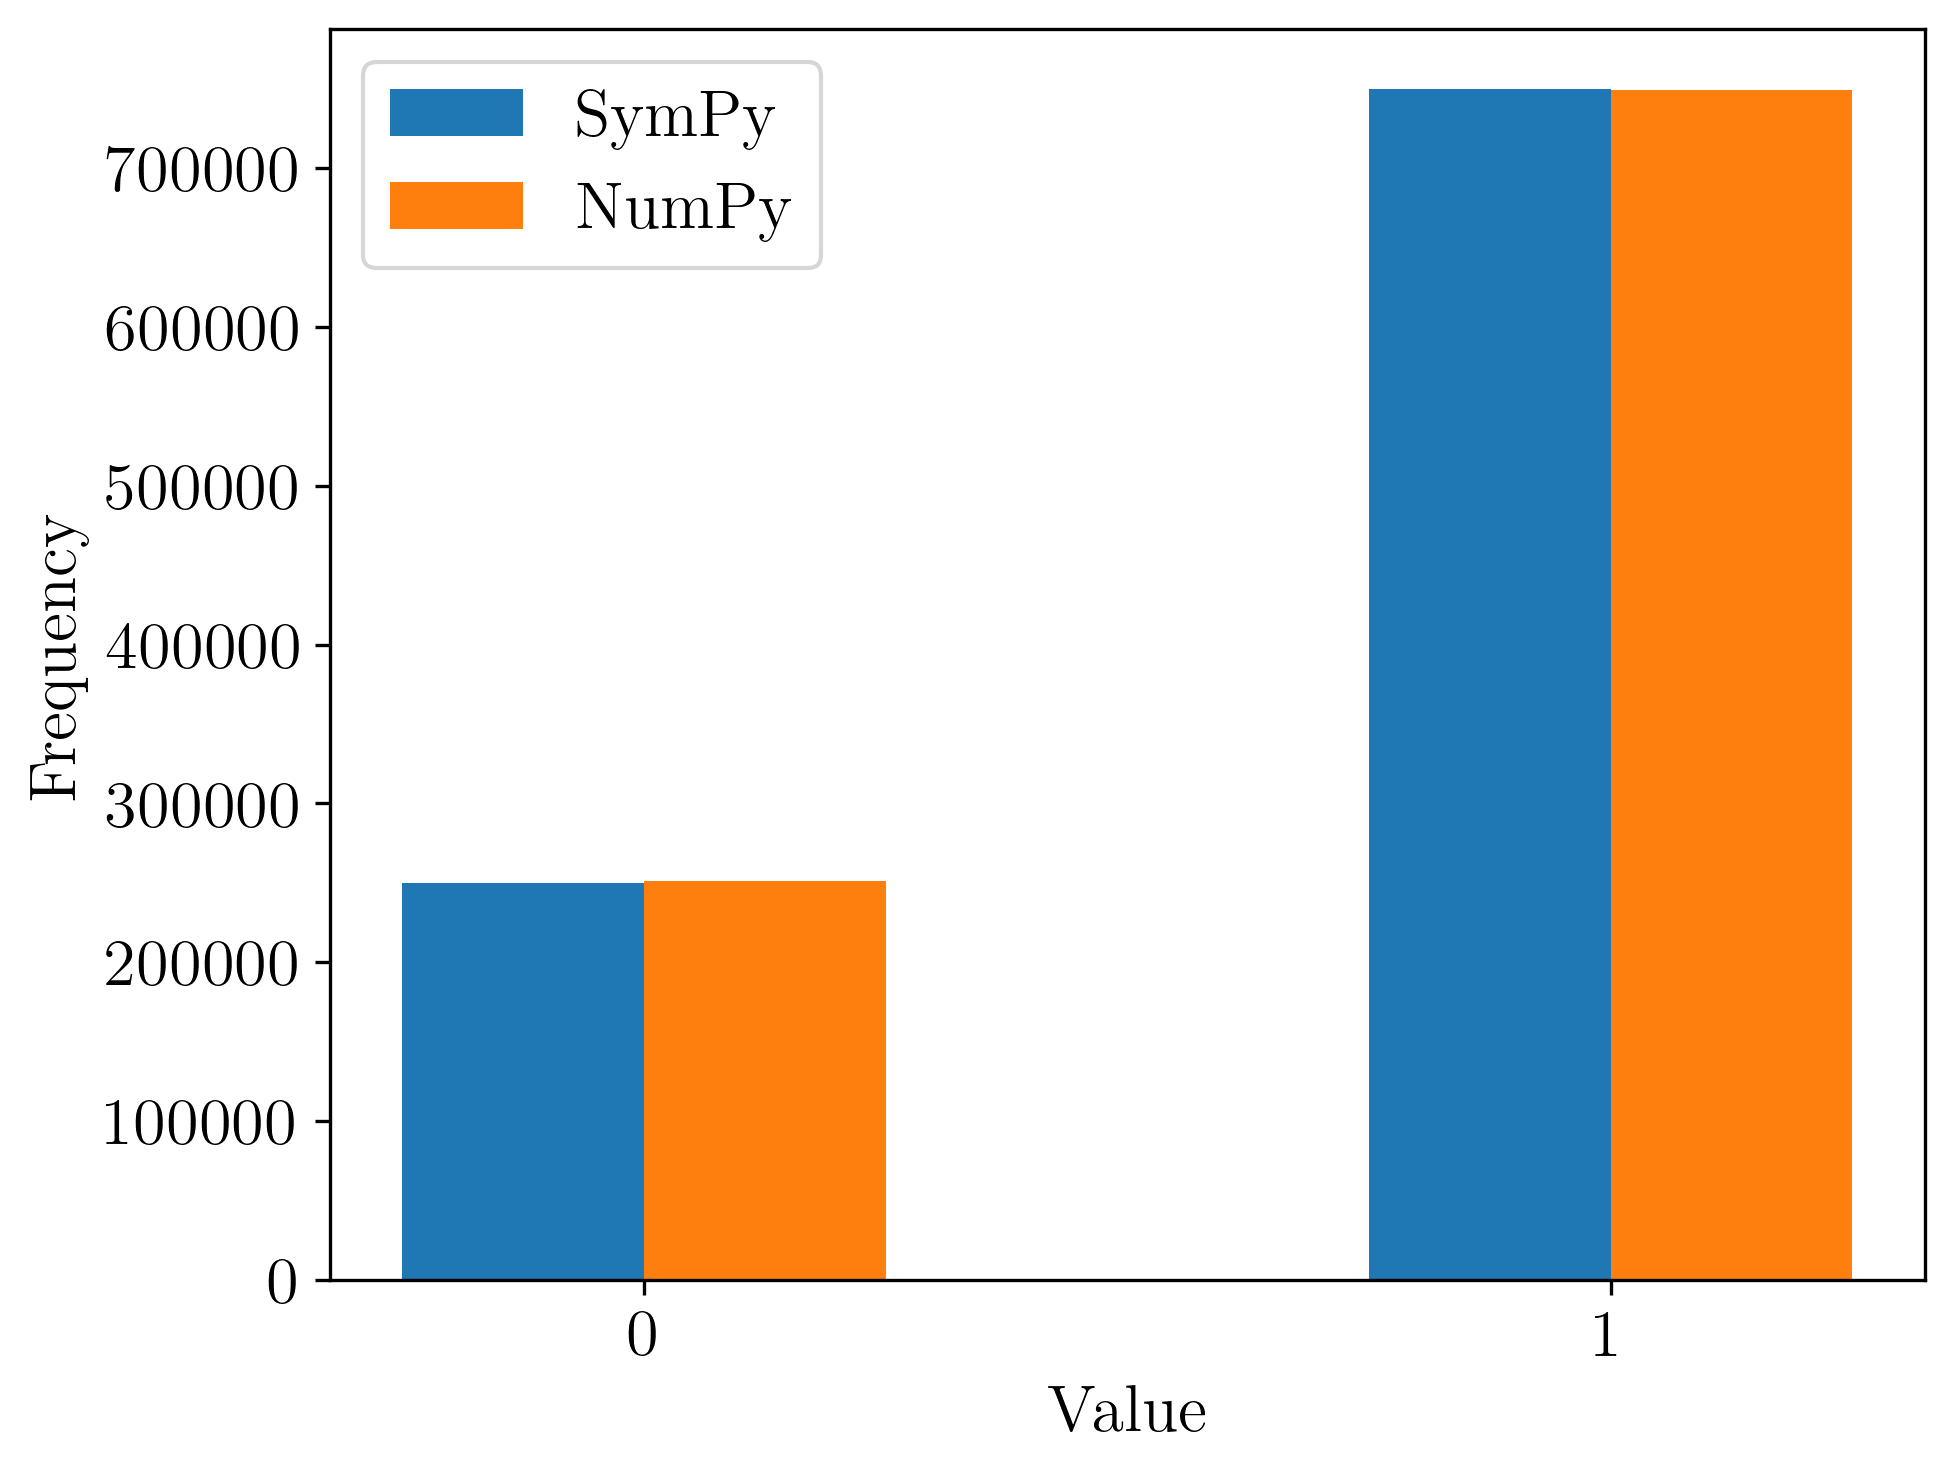
\includegraphics[width=\linewidth]{./Section/Simulation/Sim Bernoulli.png}
\caption{Simulation einer $\Ber(3/4)$-Verteilung}
\end{center}
\end{figure}
\end{minipage}
\begin{minipage}{0.5\linewidth}
\begin{figure}[H]
\begin{center}
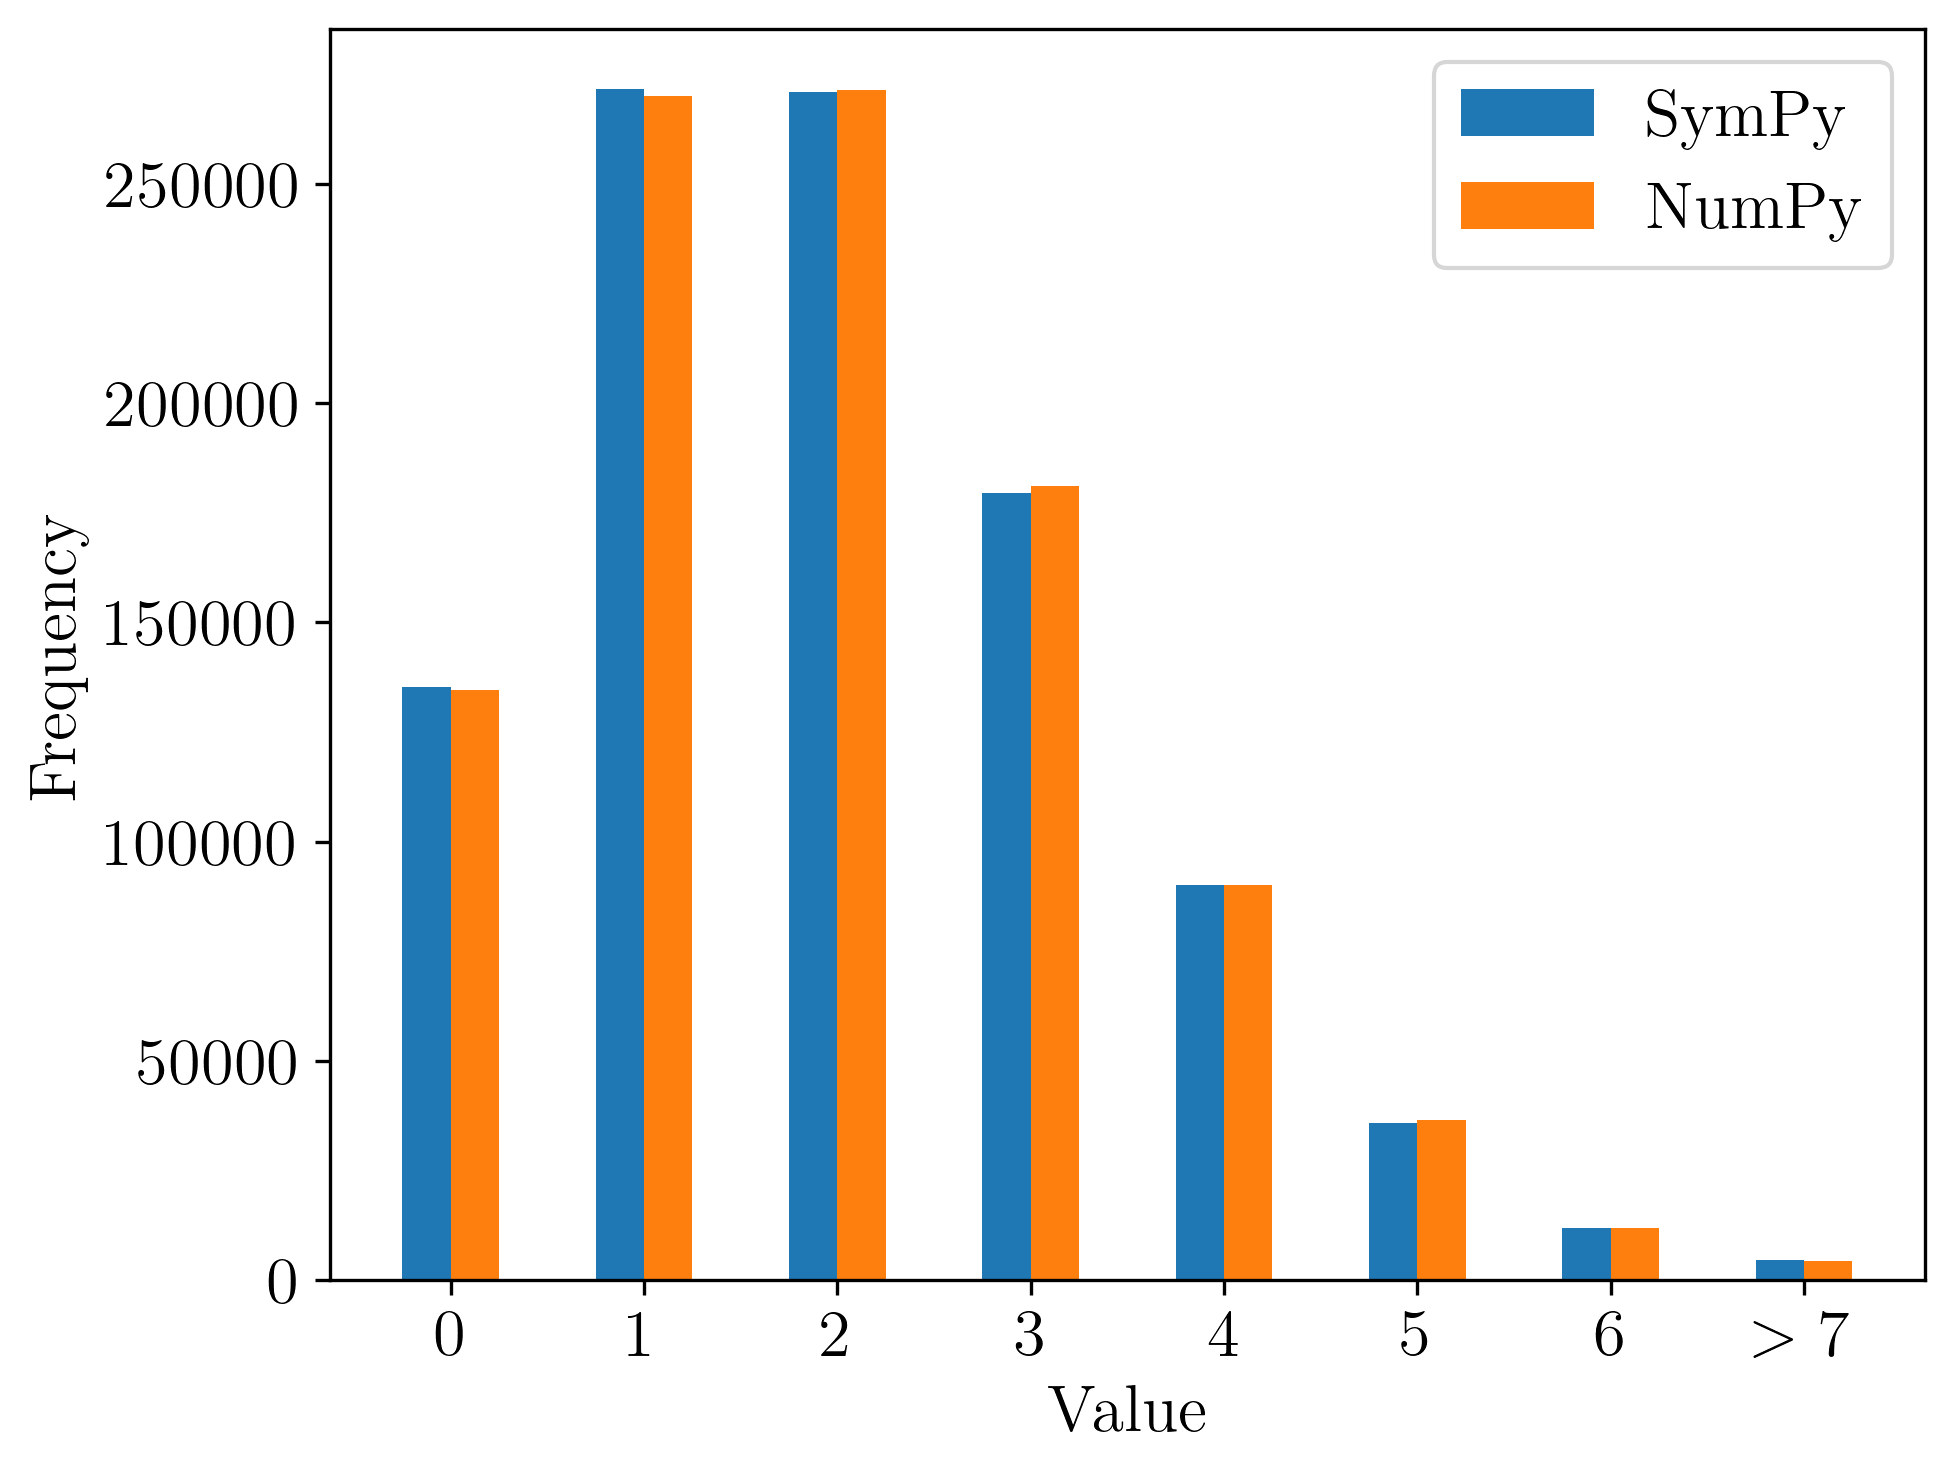
\includegraphics[width=\linewidth]{./Section/Simulation/Sim Poisson.png}
\caption{Simulation einer $\Poiss(2)$-Verteilung}
\end{center}
\end{figure}
\end{minipage}

\begin{minipage}{0.5\linewidth}
\begin{figure}[H]
\begin{center}
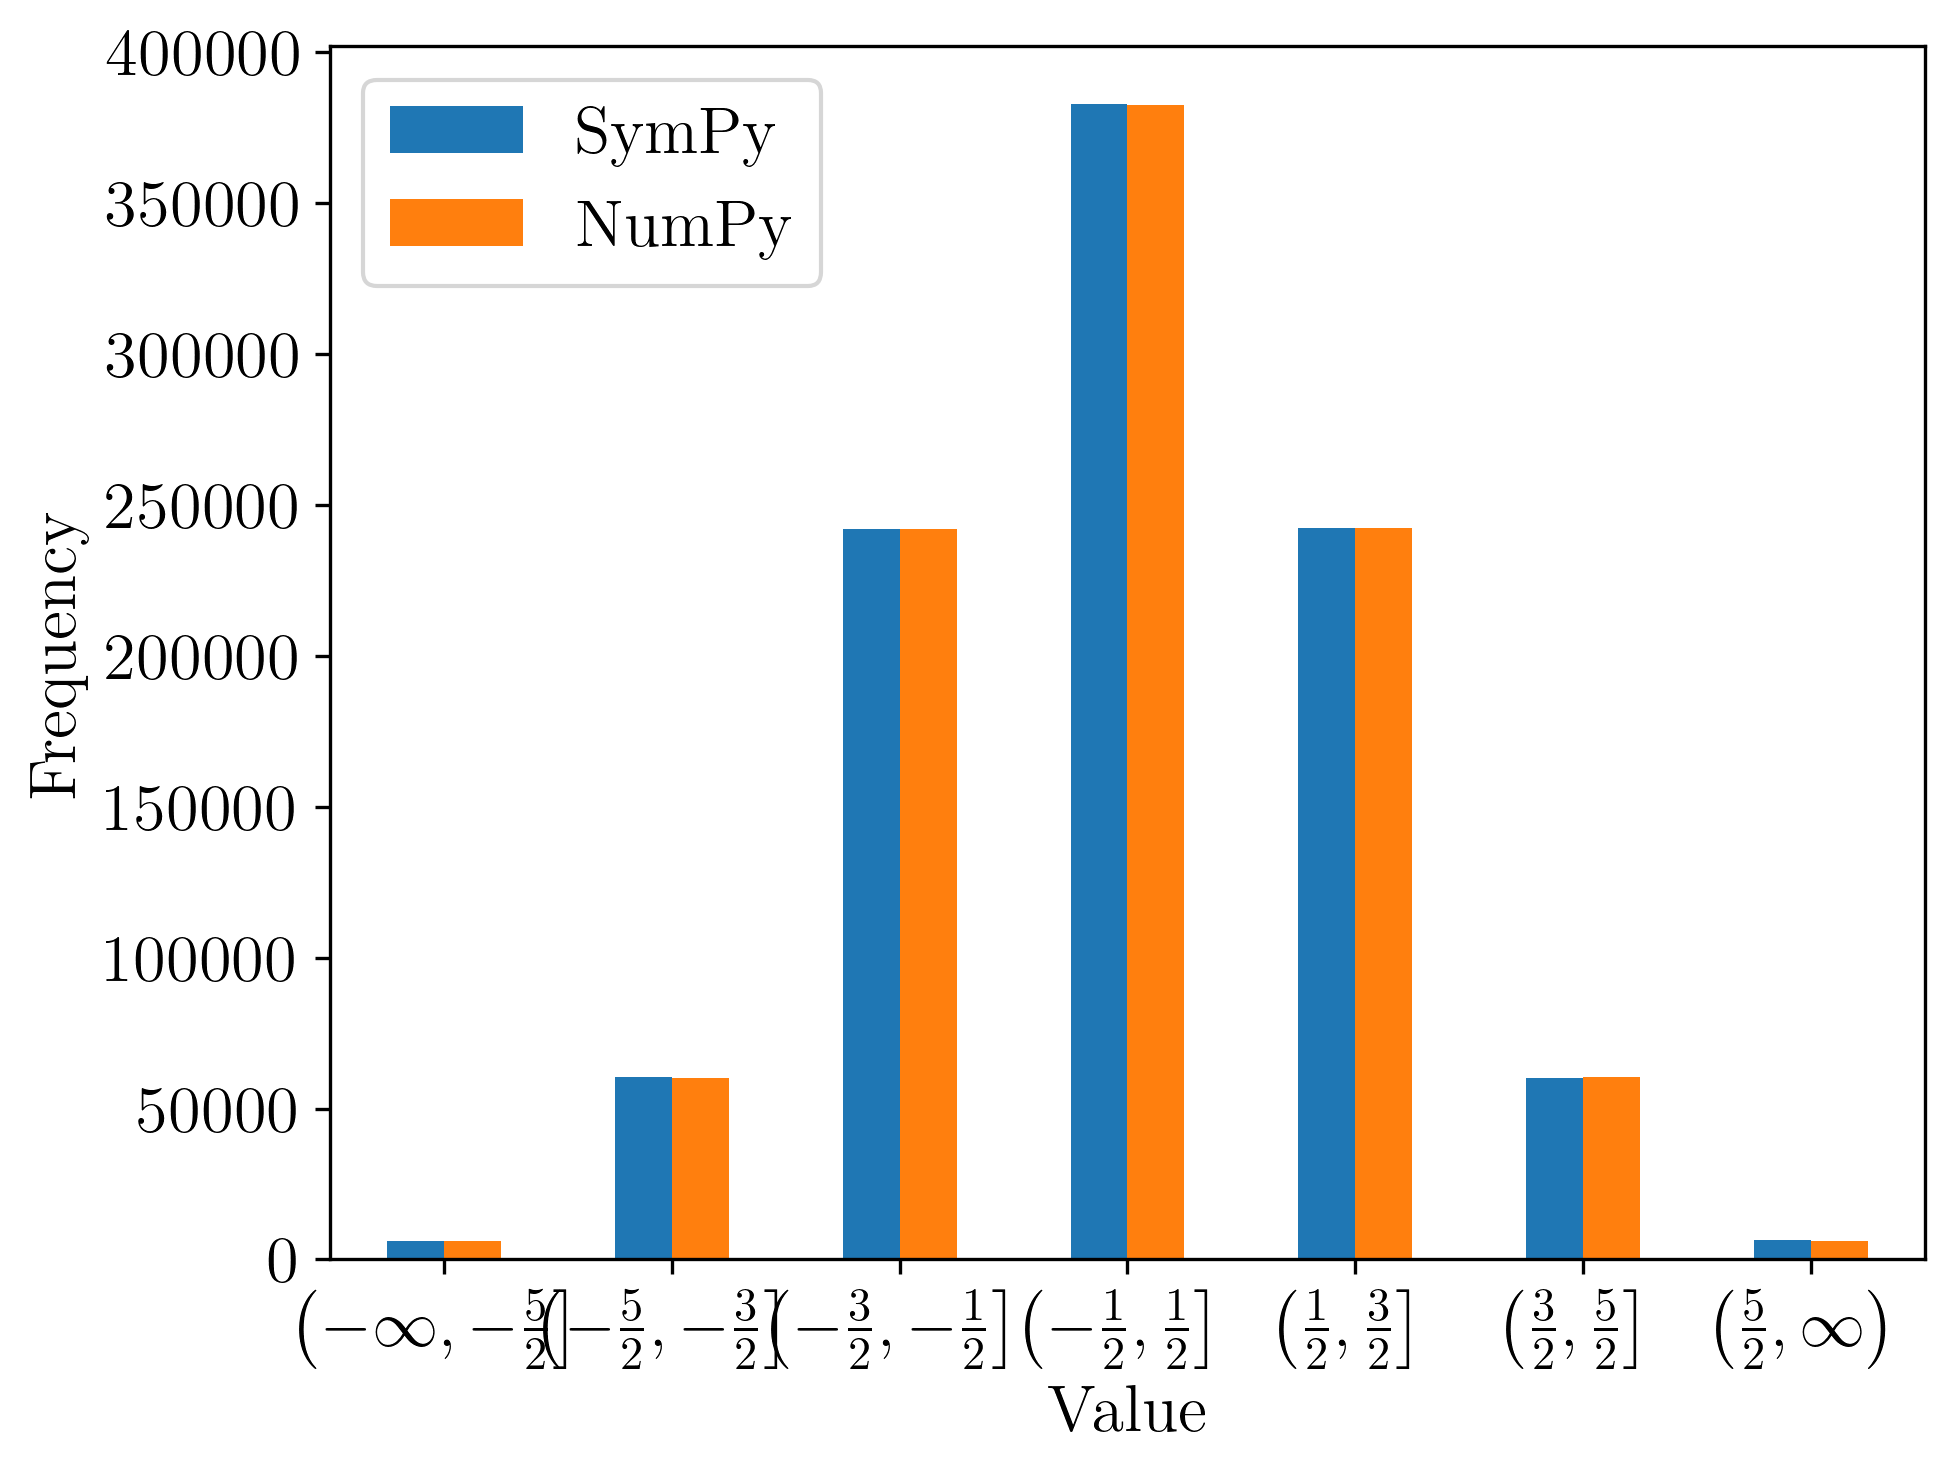
\includegraphics[width=\linewidth]{./Section/Simulation/Sim Normal.png}
\caption{Simulation einer $\Nor(0, 1)$-Verteilung}
\end{center}
\end{figure}
\end{minipage}
\begin{minipage}{0.5\linewidth}
\begin{figure}[H]
\begin{center}
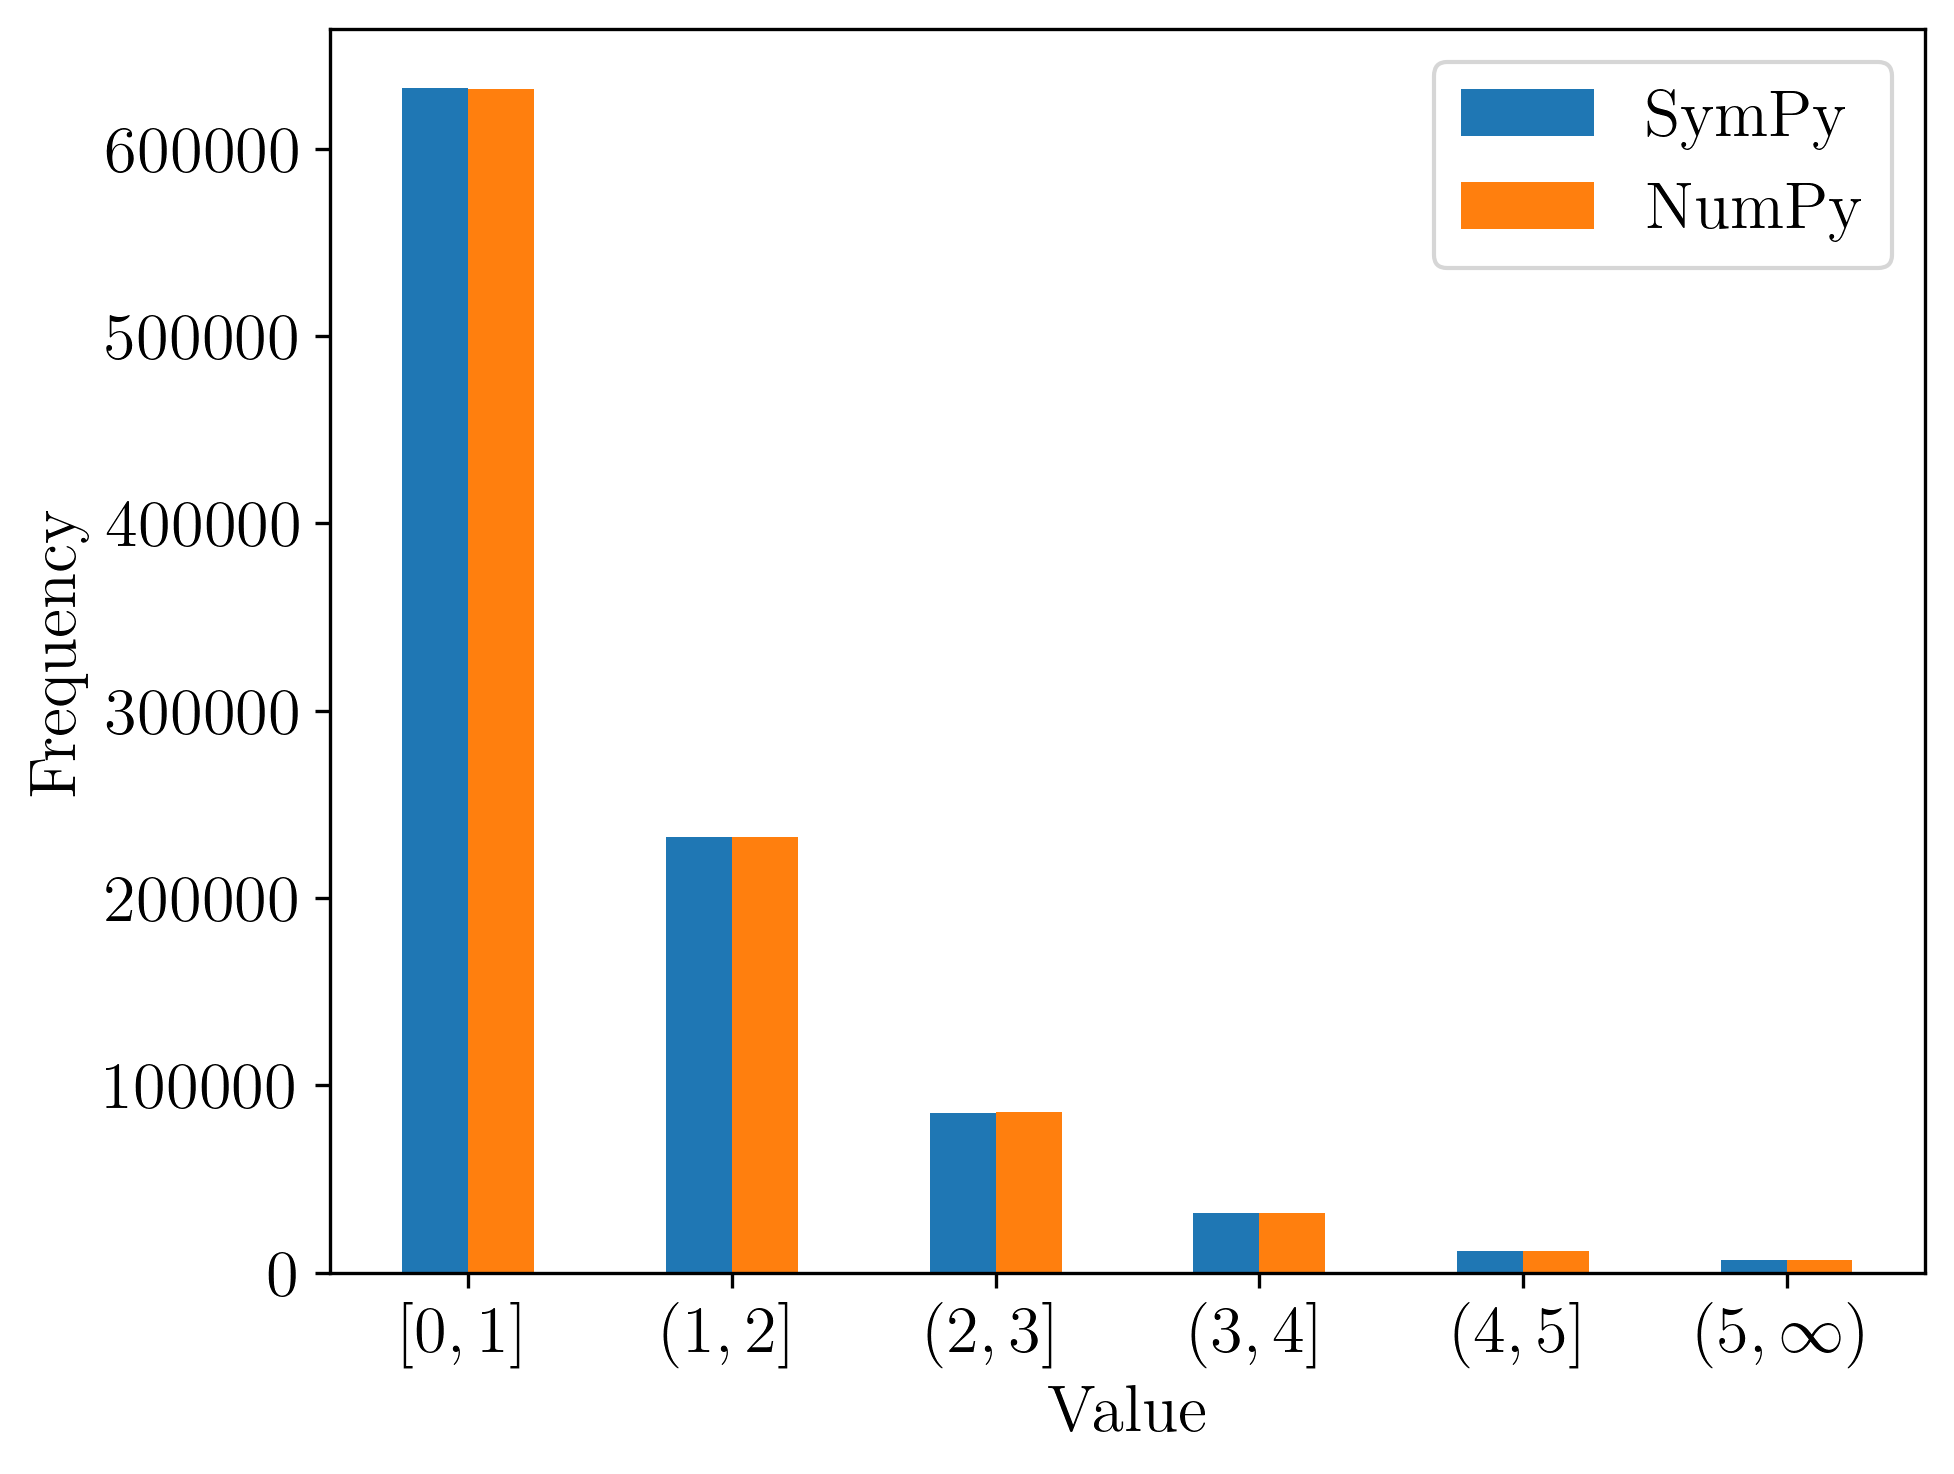
\includegraphics[width=\linewidth]{./Section/Simulation/Sim Exp.png}
\caption{Simulation einer $\Exp(3)$-Verteilung}
\end{center}
\end{figure}
\end{minipage}

Vergleicht man jeweils die Höhe benachbarter Balken miteinander, so scheint es, als würde der von uns programmierte Code genau das tun, was er soll.
\end{Beispiel}

\newpage

Als großen Vorteil gegenüber NumPy können wir die folgenden Beispiele betrachten.

\begin{Beispiel}{(Nicht-klassische Zufallsvariablen)}
Wir werden nun Zufallsvariablen simulieren, die nicht in NumPy implementiert sind und zu denen wir nur die Dichte haben.
\begin{enumerate}[label=(\roman*)]
\item Wir können an dieser Stelle das \hyperlink{Bsp:Münze}{\blue{Münzwurfbeispiel}} simulieren.
\begin{figure}[H]
\centering
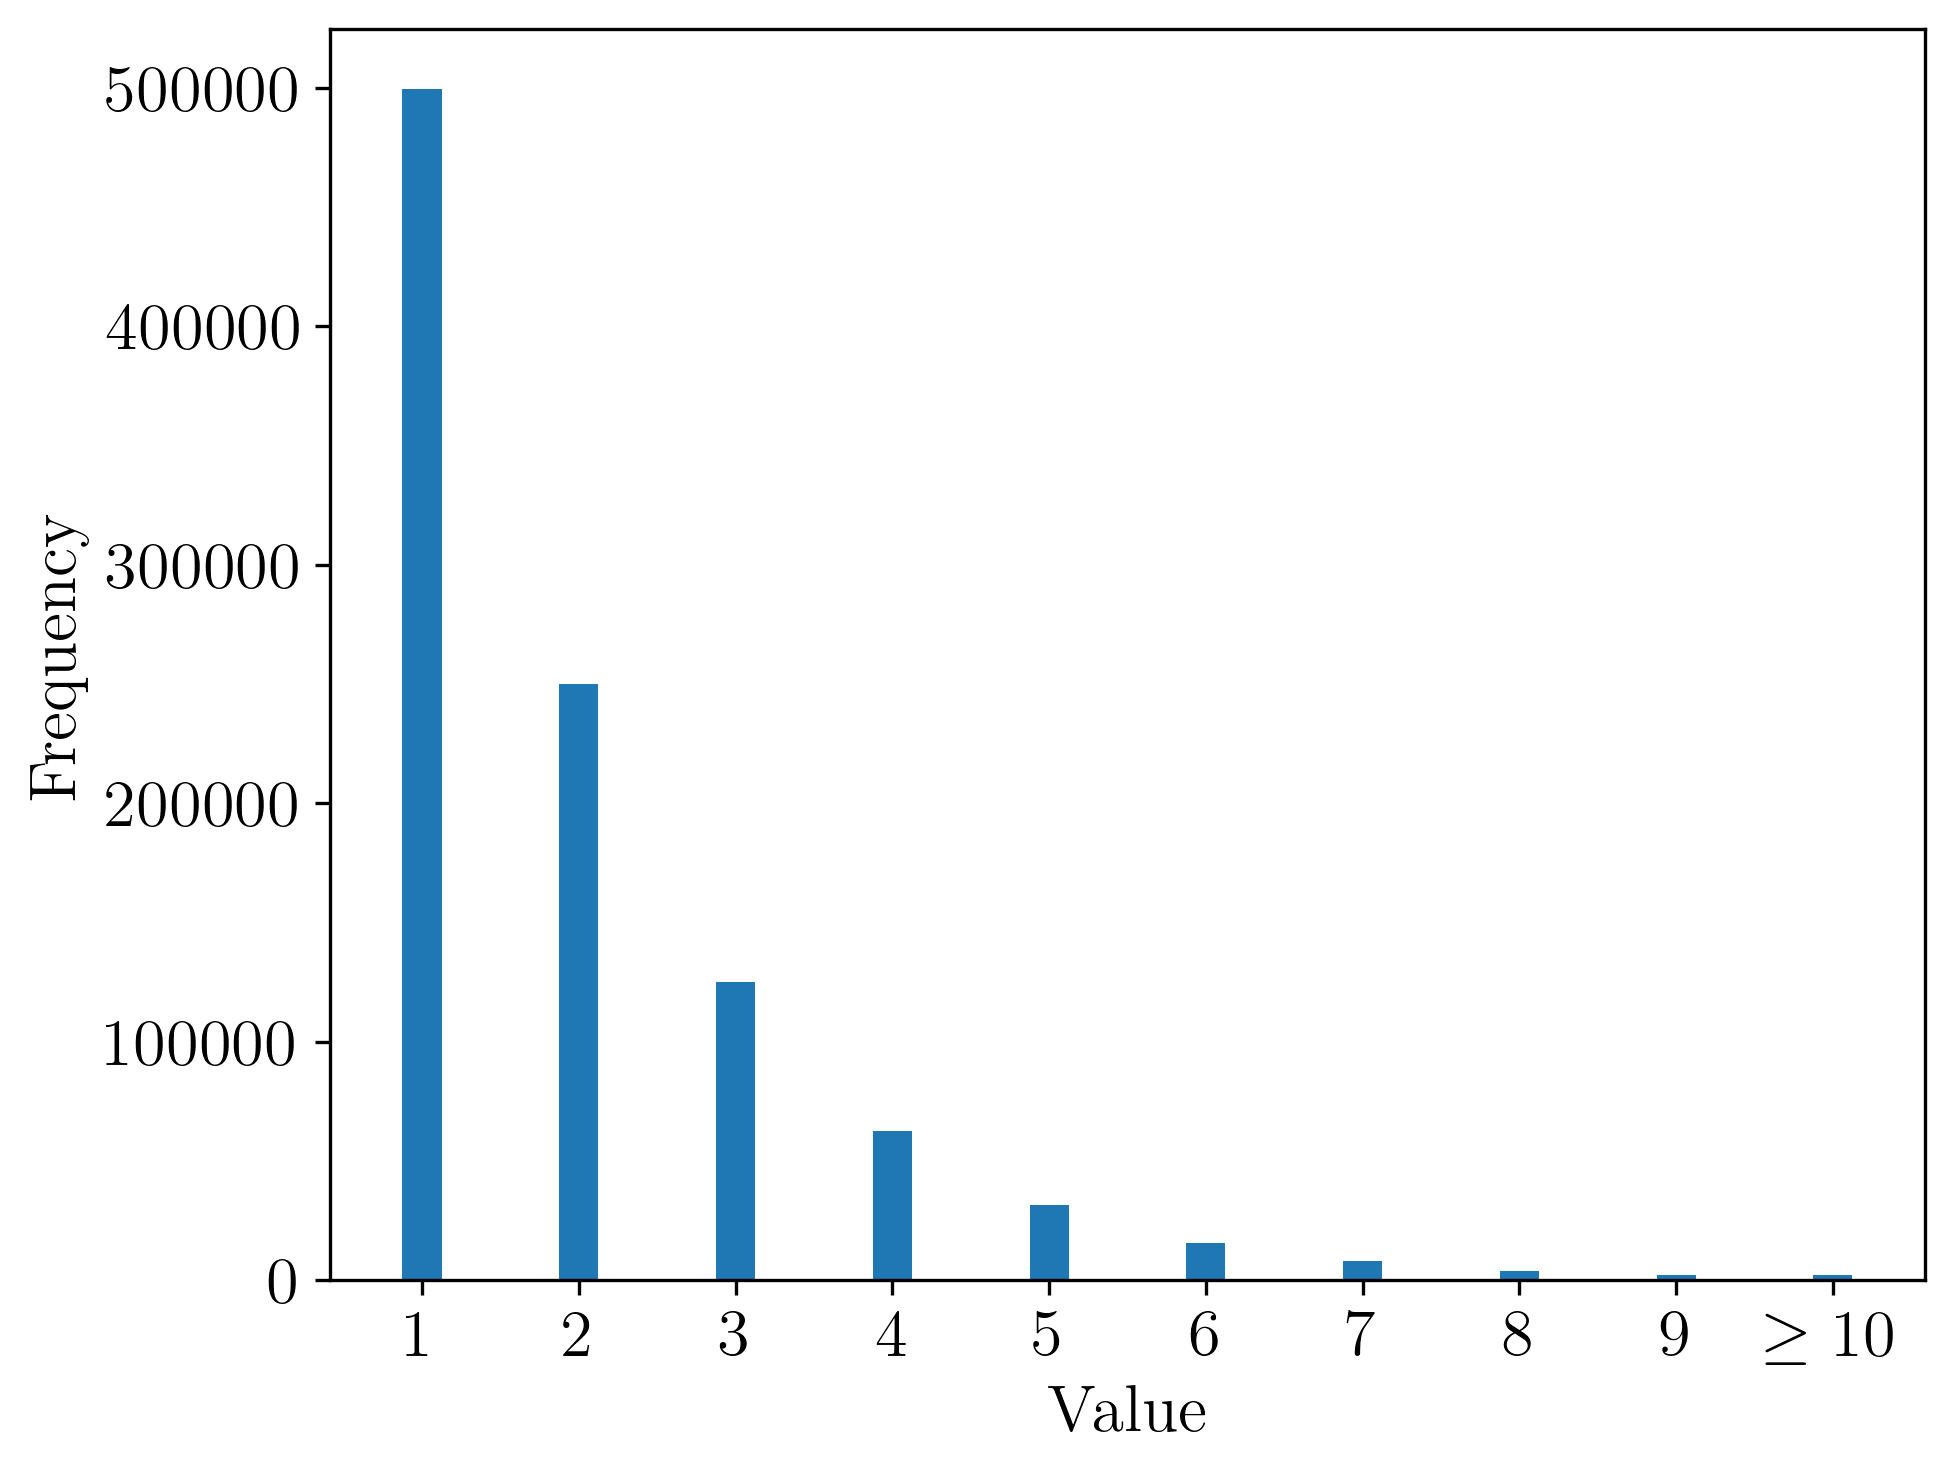
\includegraphics[width=0.5\linewidth]{./Section/Simulation/Sim Dis.png}
\caption{Simulation einer Verteilung mit Dichte $\sim 2^{- n}$}
\end{figure}
Der höchste Wert der Zufallsvariable lag bei $27$. Dieses Ereignis hat eine Wahrscheinlichkeit von
\begin{align*}
\mathbb{P}(X = 27) &= 2^{-27}\\
&= 7.4506 \cdot 10^{-9}~.
\end{align*}

\item Gegeben sei einer Verteilung mit der Dichtefunktion
\[\varphi(x) = \left(- \frac{3}{4} x^2 + \frac{3}{4}\right) \indi_{[-1, 1]}(x)~.\]
Wir können auf einfache Weise die Normiertheit nachrechnen mittels
\begin{align*}
\mathbb{P}_X(\mathbb{R}) &= \int_\mathbb{R} \left(- \frac{3}{4} x^2 + \frac{3}{4}\right) \indi_{[-1, 1]}(x) \d x\\
&= \int_{-1}^1 - \frac{3}{4} x^2 + \frac{3}{4} \d x\\
&= \left[ - \frac{1}{4} x^3 + \frac{3}{4} x \right]_{-1}^1\\
&= - \frac{1}{4} \cdot 1^3 + \frac{3}{4} \cdot 1 + \frac{1}{4} \cdot (-1)^3 - \frac{3}{4} \cdot (-1)\\
&= - \frac{1}{4} + \frac{3}{4} - \frac{1}{4} + \frac{3}{4}\\
&= 1~.
\end{align*}
Die Nullstellen von $\varphi$ sind genau an den Grenzen des Trägers, womit die Dichte überall nicht-negativ ist. Wir können nun diese Zufallsvariable simulieren und würden etwas ähnliches, wie bei der Normalverteilung erwarten, nur dass die Werte auf $[-1, 1]$ beschränkt sind.
\begin{figure}[H]
\centering
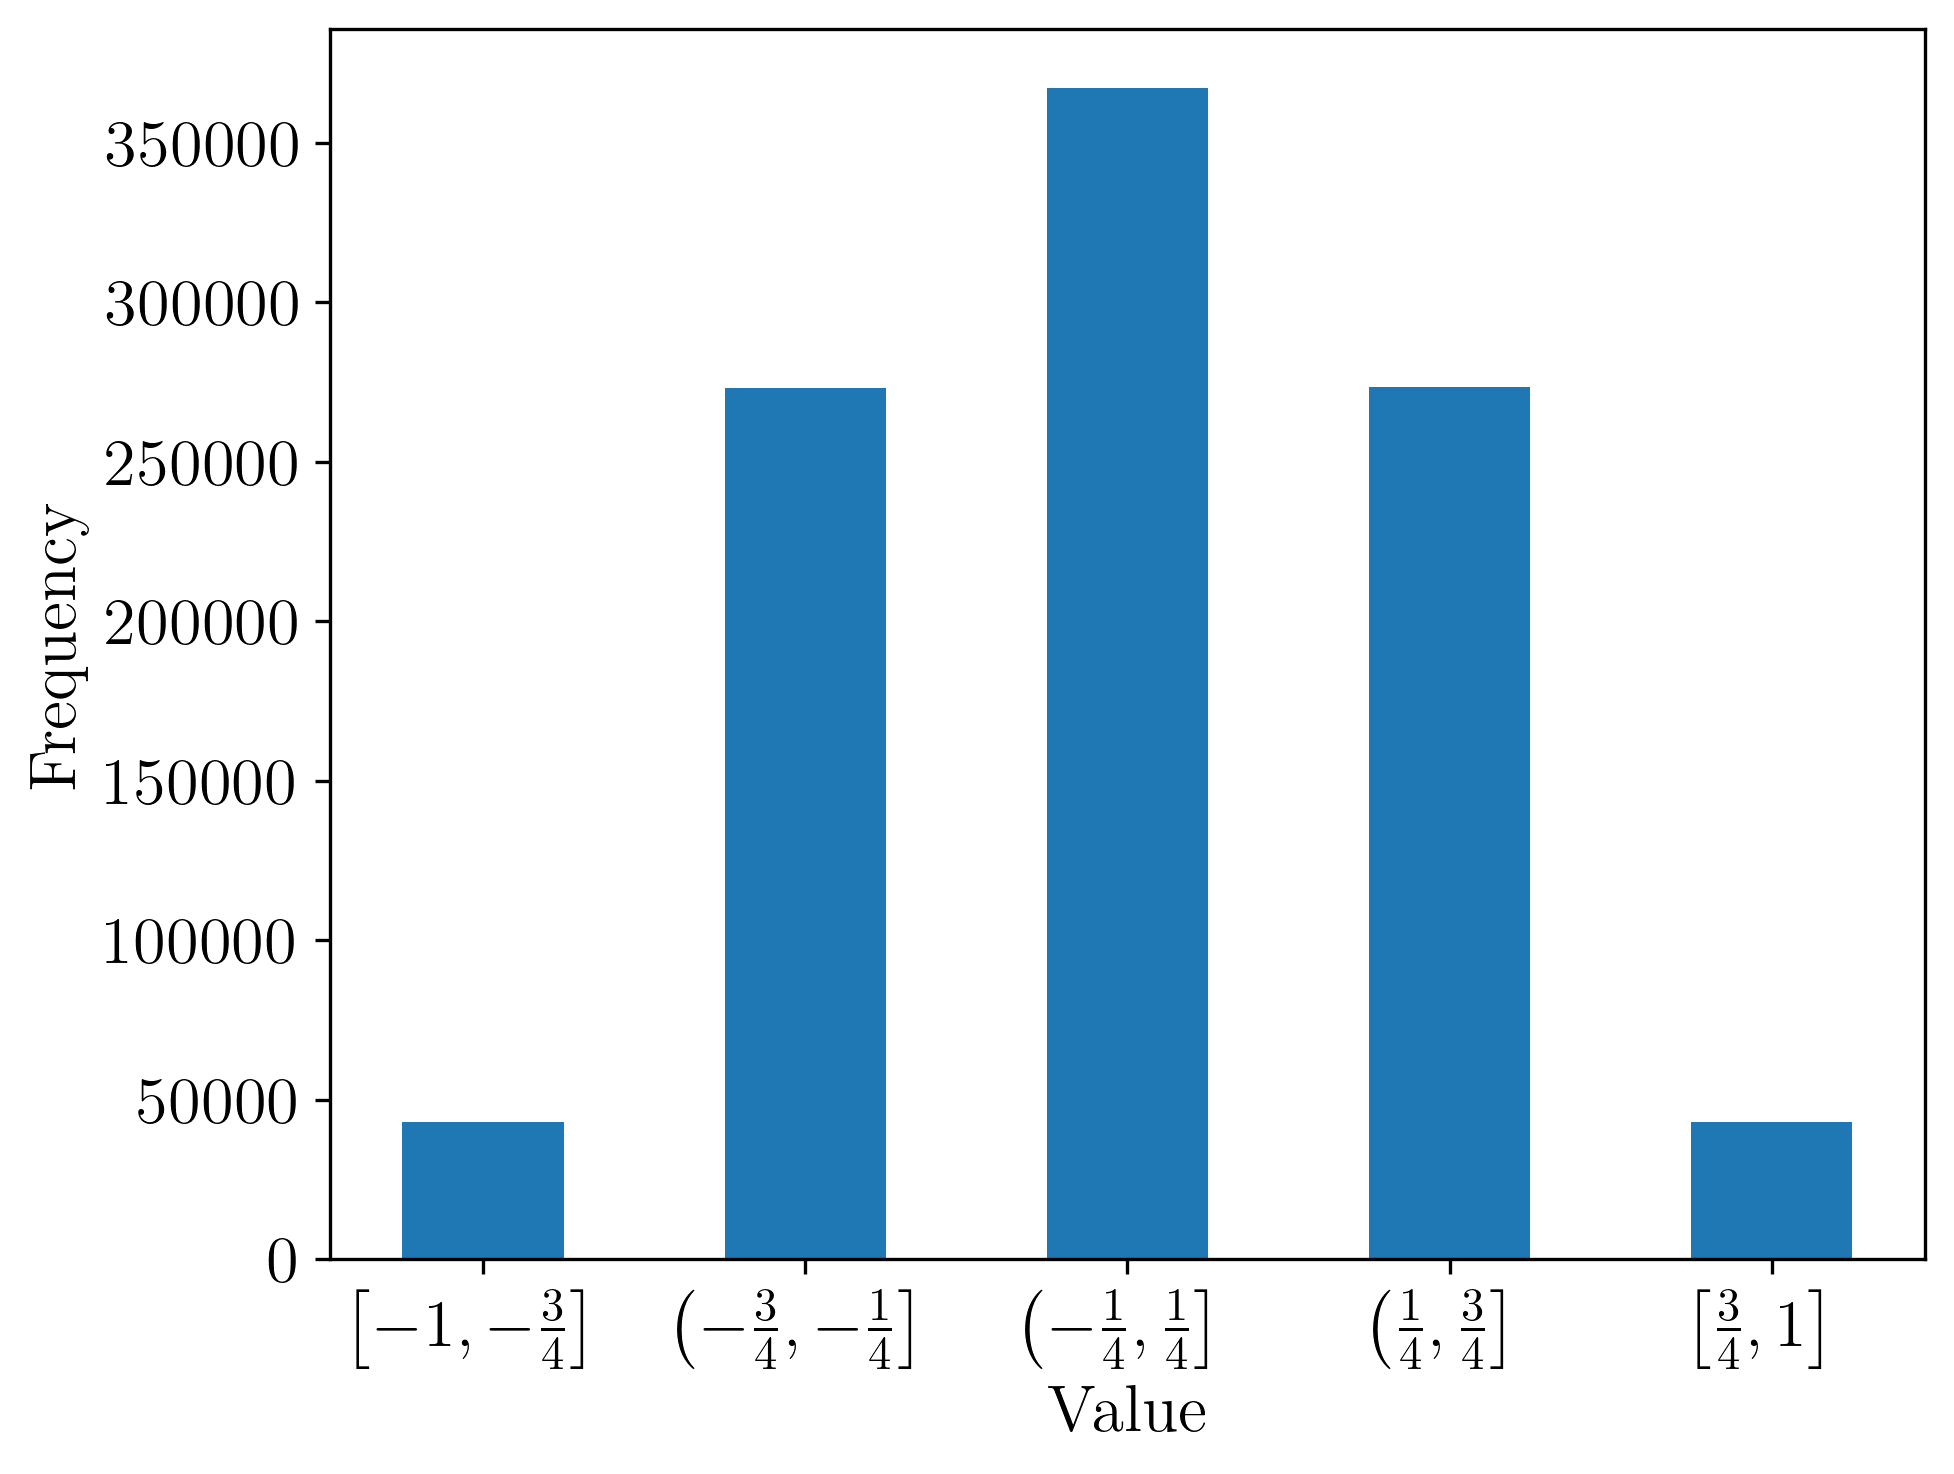
\includegraphics[width=0.5\linewidth]{./Section/Simulation/Sim Sq.png}
\caption{Simulation einer Verteilung mit Dichte $\sim - x^2$}
\end{figure}

\item Als letztes Beispiel können wir die mit der Normalverteilung verwandte, \hyperlink{Bsp:Platy}{\blue{platykurtische Verteilung}} simulieren. Wir würden wieder etwas Ähnliches zur Normalverteilung erwarten, nur dass die Enden schneller abfallen und mehr Ereignisse um die Null zentriert sind.

\begin{figure}[H]
\centering
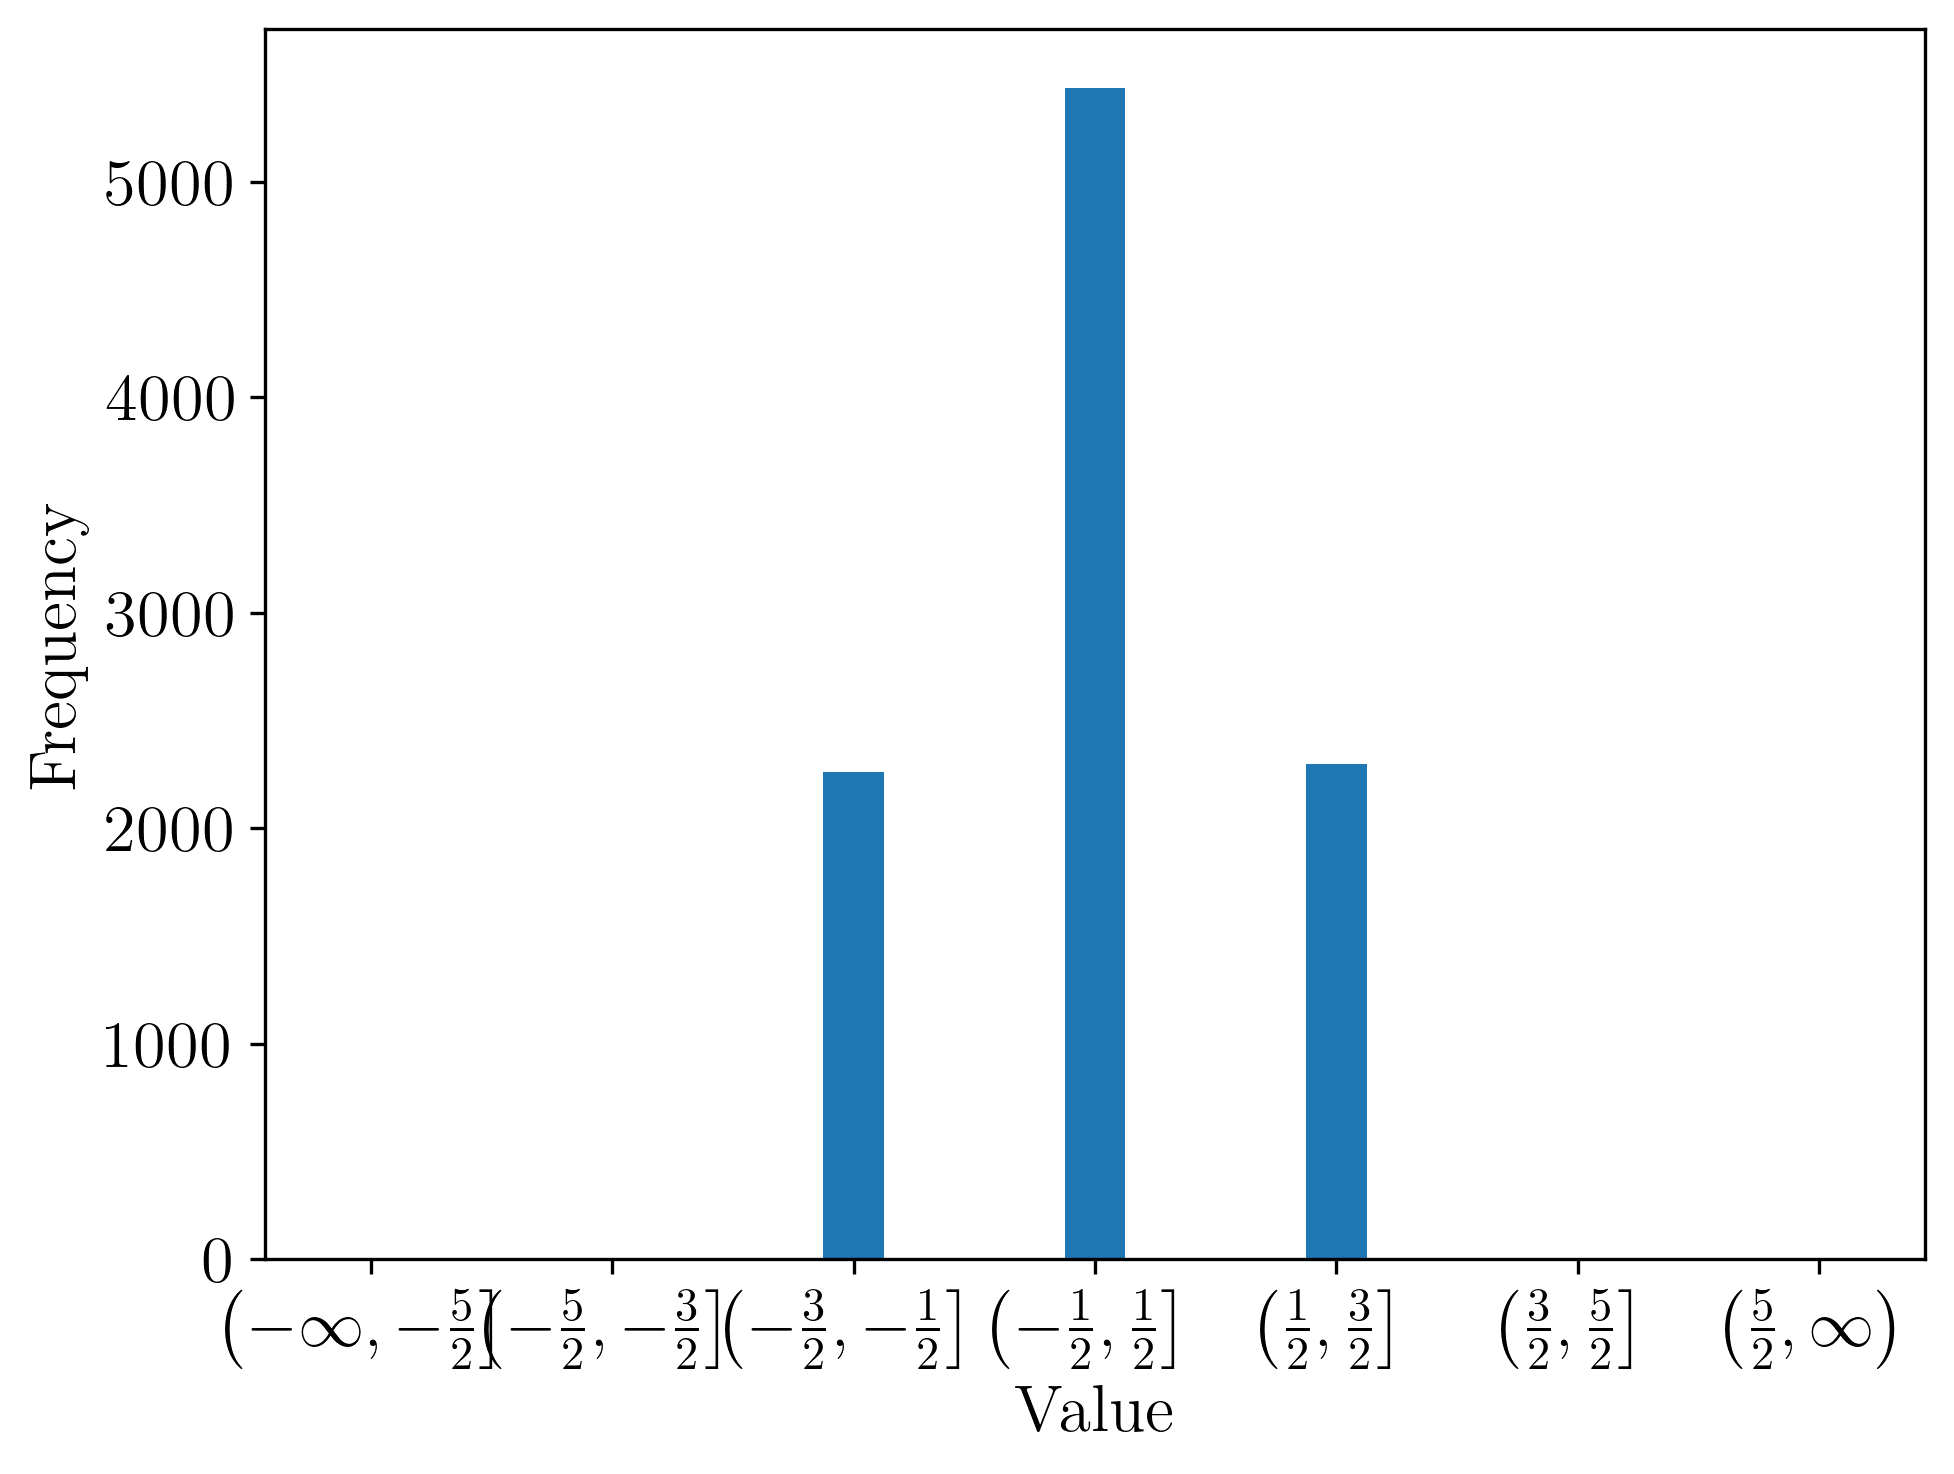
\includegraphics[width=0.5\linewidth]{./Section/Simulation/Sim Platy.png}
\caption{Simulation einer Verteilung mit Dichte $\sim \exp(- x^4)$}
\end{figure}

Da die gleiche Aufteilung auf der $x$-Achse gewählt wurde, erkennen wir genau das Vorhergesagte.
\end{enumerate}
Wir wollen es bei diesen Beispielen belassen. Insbesondere in diesem Kapitel sind der Phantasie keine Grenzen gesetzt und ich möchte Sie dazu anregen, das Programm selbst auszuprobieren.
\end{Beispiel}